\chapter{Instrumentação Industrial}

A instrumentação é relativa aos equipamentos que obtem informações acerca do estado de um determinado processo industrial. Os chamados sensores e transdutores.

A definição de sensor e transdutor está longe de ser uma unanimidade. Do ponto de vista da instrumentação, define-se:
\begin{description}
  \item[Sensor] é um elemento que gera um sinal (normalmente elétrico) a partir de uma grandeza física (calor, luz, som pressãom etc).
  \item[Transdutor] é um dispositivo que converte um sinal de uma grandeza para outra.
\end{description}

De onde se tira que todo sensor é um transdutor, mas não o contrário. Em geral os sensores se utilizam de transdutores para converter uma grandeza específica para outra mais facilmente manipulável.

Outra classificação normalmente usada é a de sensores passivos ou ativos:
\begin{description}
  \item[Sensores ativos] geram um sinal de saída sem a necessidade de alimentação externa. Exemplos: termopar, célula fotoelétrica.
  \item[Sensores passivos] requerem uma entrada de energia para gerar um sinal de saída. Exemplos: Termoresistência, sensor capacitivo.
\end{description}

A maioria dos sensores industriais são passivos.

Outra classificação bastante útil é a de sensores discretos ou contínuos:

\begin{description}
  \item[Sensores discretos] geram uma saída discreta, normalmente binária -- do ponto de vista da saída elétrica agem como chaves e são comumente chamados de sensores.
  \item[Sensores contínuos] geram uma saída que varia continuamente em função da entrada. Pode ser composto por um único transdutor (um resistor por exemplo).
\end{description}

Um complicador é que alguns textos técnicos apresentam uma confusão de sensores e transdutores com sensores discretos (chamados simplesmente de sensores) ou contínuos (chamados erroneamente de transdutores). Portanto deve-se tomar cuidado com o significado destes termos.

\section{Sensores discretos}

Como citado, a maioria dos sensores discretos industriais são chaves elétricas. Neste caso diferenciam-se os sensores de contato, que são chaves eletromecânicas; os sensores de proximidade, que detectam a presença de algum objeto sem tocá-lo; e as chaves de processo.

\subsection{Sensores de contato}
Do ponto de vista da instrumentação, qualquer chave presente no nível 1 da pirâmide que gera sinais lidos no nível 2 realizam logicamente o mesmo tipo de função. Daí que se consideram como sensores de contato:
\begin{description}
  \item[Botoeiras] ou botões, acionados pelo operador do processo.
  \item[Chaves de fim de curso] que são acionadas mecanicamente por algo no processo.
\end{description}

As botoeiras podem ter diversos formatos e funções, vide a figura~\ref{fig:botoeiras}.
\begin{figure}
  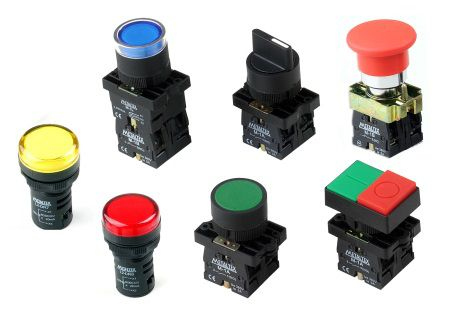
\includegraphics{figuras/botoeiras}
  \caption{Diversos tipos de botoeiras.}\label{fig:botoeiras}
\end{figure}

\begin{figure}
  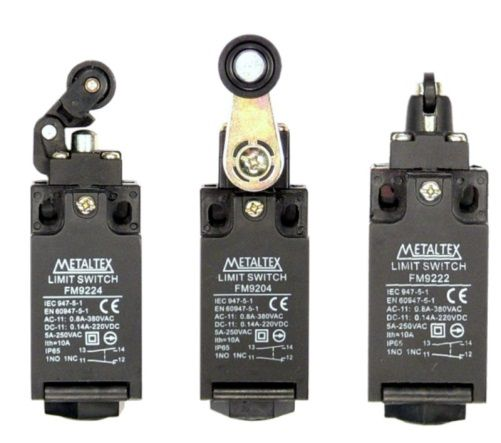
\includegraphics{figuras/fim-de-curso}
  \caption{Exemplos de chaves de fim de curso.}\label{fig:fim-de-curso}
\end{figure}

\subsection{Sensores de contato}

\subsection{Chaves de processo}

\section{Sensores Contínuos}

\section{Transmissão de dados, aterramento e blindagem em instrumentação.}
